\begin{figure*}[t!]
    \centering
    \begin{subfigure}[t]{0.5\textwidth}
        \centering
        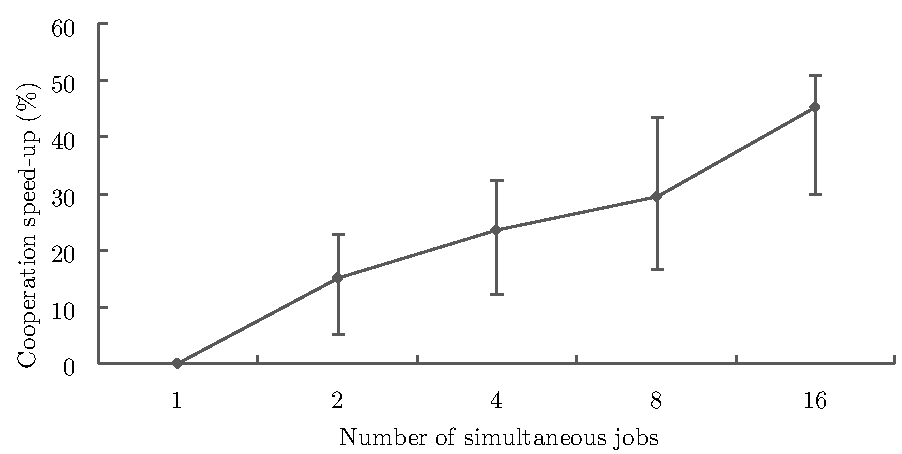
\includegraphics[width=8cm,height=4cm]{fig/randomized-pthreads.pdf}
        \caption{Pthreads implementation}
        \label{fig:pthread}
    \end{subfigure}%
    ~ 
    \begin{subfigure}[t]{0.5\textwidth}
        \centering
        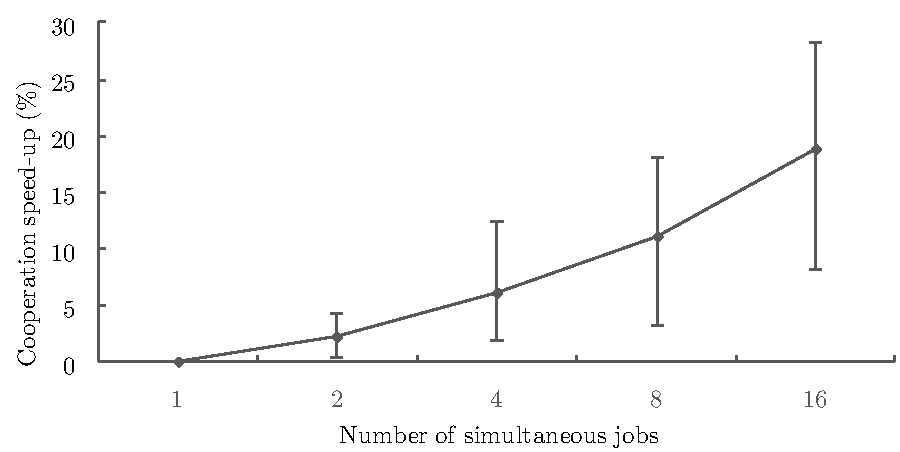
\includegraphics[width=8cm,height=4cm]{fig/randomized-tbb.pdf}
        \caption{Intel$^{\mbox{\tiny\textregistered}}$ Threading Building Blocks (TBB) implementation}
        \label{fig:tbb}
    \end{subfigure}
    \label{fig:randomized}
    \caption{The benefit from cooperation increases with contention. Each observation is 100 jobs (100 tasks each) run both with and without cooperation. The line represents the mean throughput (time to job completion) while error bars represent the maximum and minimum speed-ups we observed. Of note, we did not observe our mechanism harming performance.}
\end{figure*}